
\normalsize\chapter{PROPOSED SYSTEM}
The proposed methodology combines two components: the design of a smart bin utilising IoT and waste classification using Convolutional Neural Networks (CNN), Random Forests, and Gaussian Naive Bayes algorithms.
\section{Classification of Waste}
\par Based on the dataset, the garbage that has gathered in the bin is divided into plastic and non-plastic wastes. Python is being used in this project to train and test datasets for a variety of machine learning models. Sklearn is the most practical Python machine learning library since it offers a useful machine learning tool.
It is utilised for dimensionality reduction, clustering, regression, and classification.\\
\begin{figure}
    \centering
    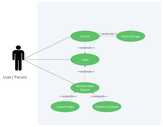
\includegraphics{b1.jpg}
    \caption{Block diagram of waste classification}
    \label{Block diagram of waste classification}
\end{figure}
\subsection{Data Collection}
The images were collected from Public GitHub dataset
which are used for classification of waste. This
dataset contains 4455 images of wastes. In 4455 images,
2410 images of plastic and 2045 images of nonplastic.
Previous works shows that large dataset provide
high accuracy.
\subsection{Data Augmentation}
By generating modified data from the original, data augmentation is used to artificially increase the size of a training set. Both the training set's size and performance can be increased by doing so.
\subsection{Testing and Training}
Three models were trained and tested using 4455
images of plastic and nonplastic wastes. The data
was split into 80\% (3564 images) for training and
20\% (891 images) for testing.
\subsection{Evaluation}
It was critical to compute the metrics accuracy, precision, recall, F1-score, and plot its ROC based on the metrics TP, TN, FP, and FN in order to assess three models.
\subsubsection{Calculation of the confusion matrix}
TP, TN, FP, and FN are all represented in matrix form.
\begin{figure}
    \centering
    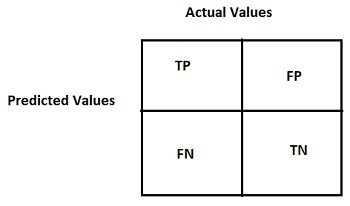
\includegraphics{v7.jpg}
    \caption{Confusion Matrix}
    \label{Confusion Matrix}
\end{figure}

\begin{itemize}
    \item True Positive (TP): True Positive (TP): Both the actual and anticipated positive values are equal in number.
\item False Positive (FP): The number of times negative values were incorrectly predicted to be positive.
\item True Negative (TN): Actual negative values have the same number as expected negative values.
\item False Negative (FN): The percentage of incorrectly interpreted negative numbers as positives
\end{itemize}
\subsubsection{Calculation of parameters}
After obtain the values of TP,FP,TN,FN from confusion
matrix, the following calculation was performed.\\
\text{1. Accuracy}\\
\par The percentage of values that were successfully categorised is calculated using accuracy. How frequently our classifier is accurate says it all. It is calculated as the total of all actual values divided by the total values.
\begin{center}
    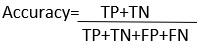
\includegraphics[]{V1.jpg}
\end{center}
\text{2. Precision}
\par The ability of the model to classify positive values correctly is calculated with precision. These results are obtained by dividing the actual positives by the total number of expected positives.
\begin{center}
    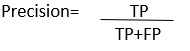
\includegraphics[]{V2.jpg}
\end{center}
\text{3. Recall}
\par It is employed to determine the model positive values' capacity for prediction. How frequently does the model correctly forecast positive values? The genuine positives are calculated by dividing them by the total number of true positives.
\begin{center}
    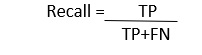
\includegraphics[]{V3.jpg}
\end{center}
\text{4. F1-Score}
\par It is Recall and Precision's harmonic mean. When you must take into account both Precision and Recall, it is helpful.
\begin{center}
    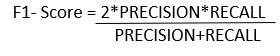
\includegraphics[]{V4.jpg}
\end{center}
\text{5. ROC}
\par ROC, which stands for receiver operating characteristic, is shown against TPR and FPR for various thresholds on the graph. FPR grows because TPR likewise rises.
\section{IoT Based Smart Bin}
No one uses the trash can since it is so filthy around the basket and people are afraid to touch the lid. As a result, the smart bin prototype can use an ultrasonic sensor to recognise when someone approaches the basket and open itself. An autonomous decomposition approach is employed to prevent disease spread through hospital waste collection and traffic jams brought on by trucks.
\subsection{Automatic Decomposition}
This prototype has an ultrasonic sensor that can measure the waste level. A controller based on the Internet of Things is connected whenever the level is more than 80 \%. It starts the suction pump's operation by opening the valve that connects to the basket's bottom.
The level is continuously monitored by an ultrasonic sensor until the container is completely empty. The valve closes and the suction pump stops once the container is empty. In order to burn off the waste, it is pushed into an incinerator. So the garbage decomposes automatically and maintain the environment clean.
FFirst, use the Arduino IDE to create the code for the automatic decomposition process.
Using a USB cable, the code was uploaded to the Arduino UNO after being compiled.\\
The hardware connection comes next.\\
\text{1. Connection of Ultrasonic Sensor}
\begin{itemize}
    \item Trigger pin to 2
    \item Echo pin to 3
    \item Ground pin to GND
    \item Power pin to 5V
    
\end{itemize}
\text{2. Connection of LED}
\begin{itemize}
    \item LED to 8
\end{itemize}
\text{3. Power Supply}
\begin{itemize}
    \item Power bank connected by USB cable
\end{itemize}
\begin{figure}
    \centering
    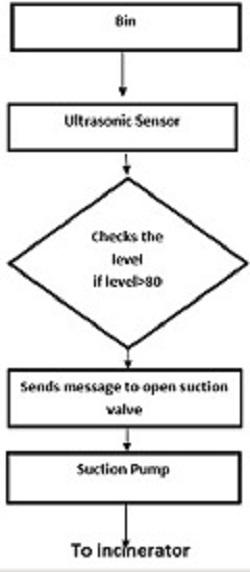
\includegraphics{b2.jpg}
    \caption{Block diagram of Smart Bin}
    \label{Block diagram of Smart Bin}
\end{figure}
\subsection{Automatic Control of Door}
\par To identify a person approaching the basket, an ultrasonic sensor is employed. It will automatically open the lid if it spots someone. It was accomplished with a motor's assistance.
Using a USB cable, code is written in the Arduino IDE and uploaded to the Arduino UNO. The hardware connectors are as follows:
\\\\
\text{1. Connection of Servo Motor}
    \begin{itemize}
        \item Signal to 7 of Arduino UNO
        \item Ground to GND
        \item Power to 3.5V
    \end{itemize}
    \text{2. Connection of Ultrasonic Sensor}
    \begin{itemize}
        \item Trigger pin to 5
        \item Echo pin to 6
        \item Ground to GND
        \item Power to 5V
    \end{itemize}
\text{3. Power Supply}
\begin{itemize}
    \item Power bank connected by USB cable
\end{itemize}



















